%==================== Appendix.tex ====================

\clearpage
\thispagestyle{plain}

\begingroup
% เนื้อหาภาคผนวก: 16pt baseline ~19.2pt ตามสเปกเล่ม
\fontsize{16pt}{19.2pt}\selectfont
\justifying
\XeTeXlinebreakskip=0pt plus 1pt minus 0.5pt
\setlength{\parindent}{1.5cm}
\setlength{\parskip}{0pt}

\indent วิธีการใช้งานในส่วนของผู้เชี่ยวชาญ เพื่อเป็นแนวทางในการใช้งานในส่วนที่ซับซ้อน และอาจทำให้สับสนในการใช้งานได้ จึงจัดทำคู่มือการใช้งานขึ้นมาเพื่ออำนวยความสะดวก

\vspace{\baselineskip}

\begin{figure}[h]
	\centering
	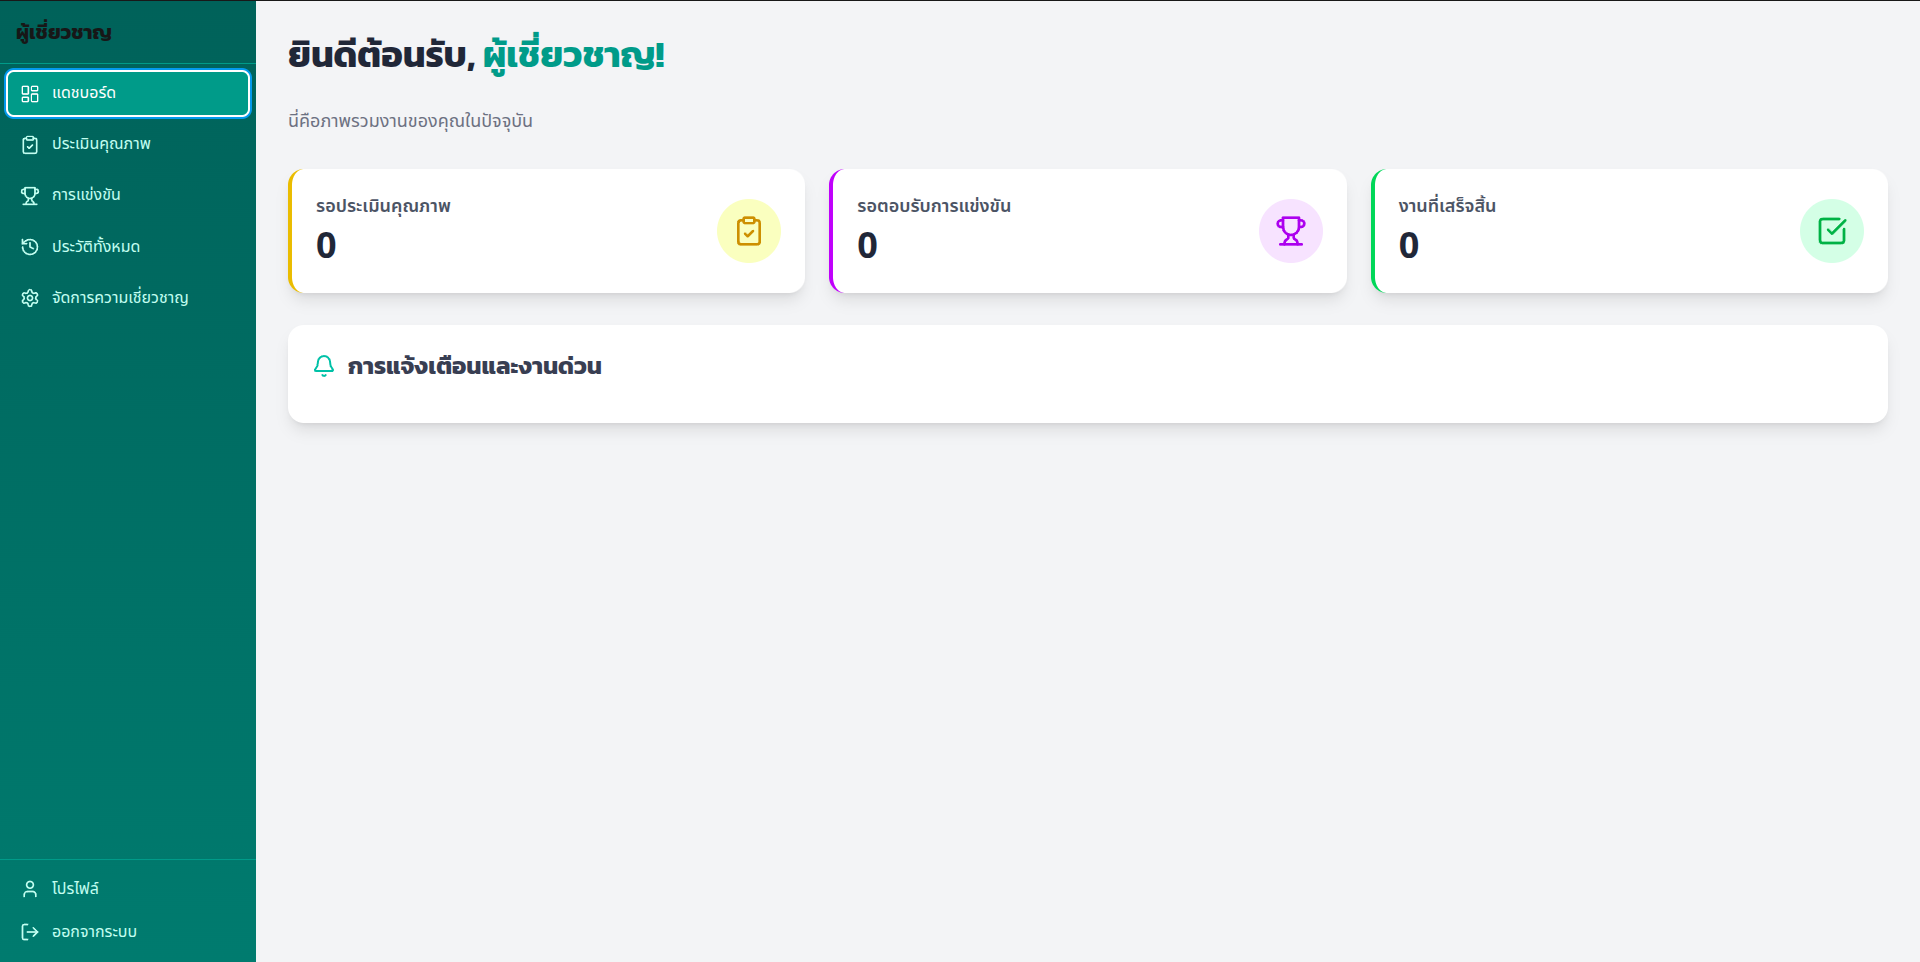
\includegraphics[width=0.8\linewidth]{EP1}
	\caption{หน้าแดชบอร์ดผู้เชี่ยวชาญ}
\end{figure}

\noindent{\bfseries\fontsize{16pt}{19.2pt}\selectfont วิธีใช้งานหน้าแดชบอร์ดผู้เชี่ยวชาญ}\par

\begin{sloppypar}
	\begin{enumerate}
		\item ใช้ดูภาพรวมงานของผู้เชี่ยวชาญแบบรวดเร็ว ได้แก่ จำนวน “รอประเมินคุณภาพ”, “รอตอบรับการแข่งขัน”, และ “งานที่เสร็จสิ้น”
		\item มีการ์ดสรุปสถิติ 3 ใบ (คลิกได้)
		\begin{enumerate}
			\item รอประเมินคุณภาพ — ลิงก์ไปที่ /expert/evaluations
			\item รอตอบรับการแข่งขัน — ลิงก์ไปที่ /expert/judging
			\item งานที่เสร็จสิ้น — ลิงก์ไปที่ /expert/history
		\end{enumerate}
		\item ส่วน “การแจ้งเตือนและงานด่วน” จะแสดงกล่องแจ้งเตือนจำนวนงานที่ต้องทำทันที (ถ้ามี) เช่น จำนวนงานรอประเมิน และจำนวนคำเชิญเป็นกรรมการที่ยังไม่ตอบรับ
		\item ขณะโหลดจะแสดงสัญลักษณ์กำลังประมวลผล และหากไม่มีงานค้าง ระบบจะแจ้งว่า “ไม่มีงานที่ต้องดำเนินการในขณะนี้”
		\item แสดงชื่อผู้ใช้งานด้านบนเพื่อความชัดเจนว่าเป็นแดชบอร์ดของผู้เชี่ยวชาญ
	\end{enumerate}
\end{sloppypar}

\noindent{\bfseries\fontsize{16pt}{19.2pt}\selectfont ขั้นตอนใช้งาน}\par

\begin{sloppypar}
	\begin{enumerate}
		\item เข้าสู่ระบบด้วยบทบาทผู้เชี่ยวชาญ แล้วเปิด “แดชบอร์ดผู้เชี่ยวชาญ”
		\item ดูตัวเลขสรุปในแต่ละการ์ดเพื่อประเมินภาพรวมงานปัจจุบัน
		\item หากต้องประเมินงาน ให้คลิกการ์ด “รอประเมินคุณภาพ” เพื่อไปยังหน้ารายการที่ต้องประเมิน
		\item หากมีคำเชิญเป็นกรรมการ ให้คลิกการ์ด “รอตอบรับการแข่งขัน” เพื่อเข้าไปตอบรับ/ปฏิเสธ
		\item ต้องการดูผลงานที่ดำเนินการเสร็จแล้ว ให้คลิกการ์ด “งานที่เสร็จสิ้น” เพื่อดูประวัติ
		\item ตรวจสอบส่วน “การแจ้งเตือนและงานด่วน” หากมีกล่องแจ้งเตือน แนะนำให้เริ่มดำเนินการตามที่ระบุ
		\item หากตัวเลขยังไม่อัปเดตหลังดำเนินการ สามารถรีเฟรชหน้าเพื่อดึงข้อมูลล่าสุดได้
	\end{enumerate}
\end{sloppypar}

\begin{figure}[h]
	\centering
	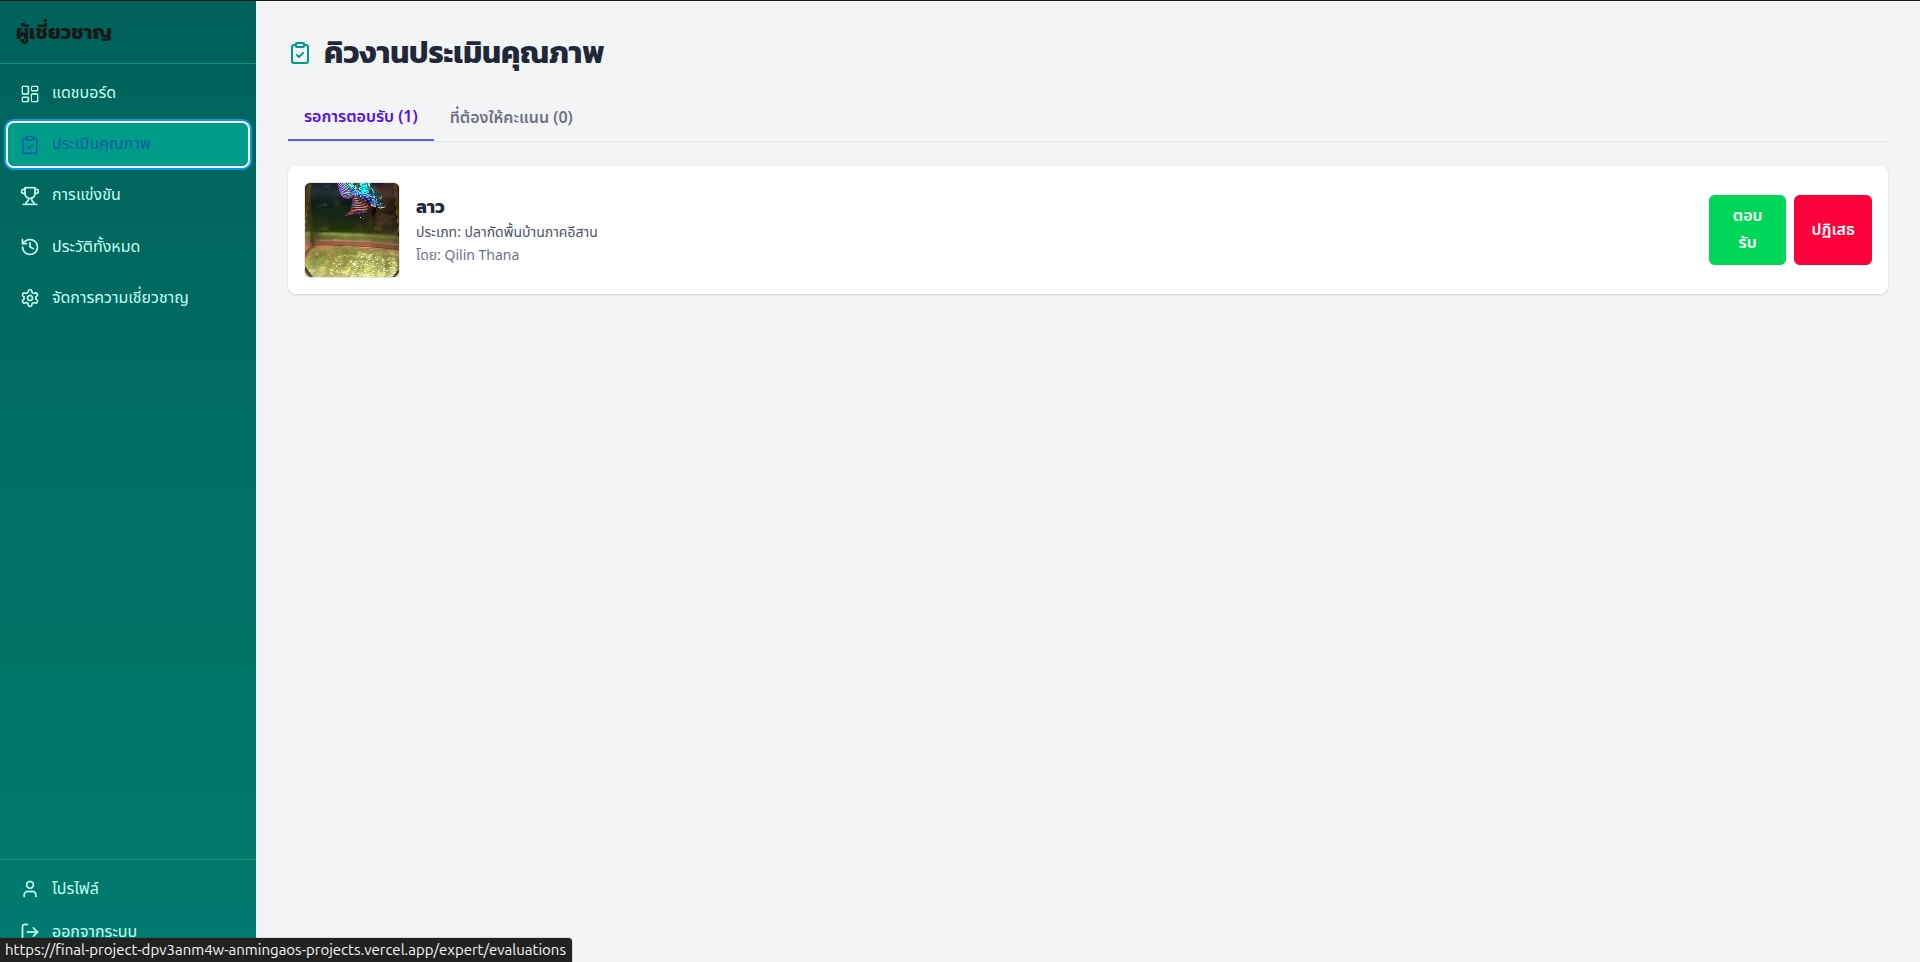
\includegraphics[width=0.8\linewidth]{EP2}
	\caption{หน้าคิวงานประเมินคุณภาพ (ผู้เชี่ยวชาญ)}
\end{figure}

\noindent{\bfseries\fontsize{16pt}{19.2pt}\selectfont วิธีใช้งานหน้าคิวงานประเมินคุณภาพ (ผู้เชี่ยวชาญ)}\par

\begin{sloppypar}
	\begin{enumerate}
		\item หน้าแสดง “คิวงานประเมินคุณภาพ” แบ่ง 2 แท็บ:
		\emph{รอการตอบรับ} (งานที่ผู้เชี่ยวชาญต้องกดรับหรือปฏิเสธ) และ
		\emph{ที่ต้องให้คะแนน} (งานที่ตอบรับแล้วและพร้อมเปิดฟอร์มให้คะแนน)
		\item แต่ละรายการจะแสดงภาพปลากัด ชื่อปลา ประเภท ผู้ส่ง และสถานะปัจจุบัน
		\item ปุ่มสำหรับงานในแท็บ \emph{รอการตอบรับ}:
		“ตอบรับ” เพื่อรับงาน, “ปฏิเสธ” เพื่อระบุเหตุผลและคืนงาน
		\item ปุ่มสำหรับงานในแท็บ \emph{ที่ต้องให้คะแนน}:
		“ให้คะแนน” เพื่อเปิดฟอร์มกรอกคะแนนและส่งผล
		\item มีสถานะระหว่างทำงาน: แสดงสัญลักษณ์กำลังโหลดเมื่อดึงข้อมูล,
		และแสดงหน้าว่างพร้อมข้อความเมื่อไม่มีรายการในคิว
		\item เมื่อดำเนินการสำเร็จ (ตอบรับ/ปฏิเสธ/ส่งคะแนน) ระบบจะแจ้งเตือนและรีเฟรชคิวอัตโนมัติ
	\end{enumerate}
\end{sloppypar}

\noindent{\bfseries\fontsize{16pt}{19.2pt}\selectfont ขั้นตอนใช้งาน}\par

\begin{sloppypar}
	\begin{enumerate}
		\item เปิดเมนู “คิวงานประเมินคุณภาพ”
		\item เลือกแท็บที่ต้องการ
		\begin{enumerate}
			\item แท็บ “รอการตอบรับ”: ตรวจรายละเอียด แล้วกด “ตอบรับ” หรือ “ปฏิเสธ”
			\item แท็บ “ที่ต้องให้คะแนน”: กด “ให้คะแนน” เพื่อเปิดฟอร์ม
		\end{enumerate}
		\item หากปฏิเสธ ระบบจะเปิดหน้าต่างให้กรอกเหตุผล กดยืนยันเพื่อส่งกลับคิว
		\item หากให้คะแนน ให้กรอกคะแนนในฟอร์มให้ครบ แล้วกด “ส่งคะแนน”
		\item ตรวจสอบข้อความแจ้งเตือนความสำเร็จ จากนั้นรายการจะย้ายสถานะ/หายจากคิวตามเงื่อนไข
	\end{enumerate}
\end{sloppypar}


\begin{figure}[h]
	\centering
	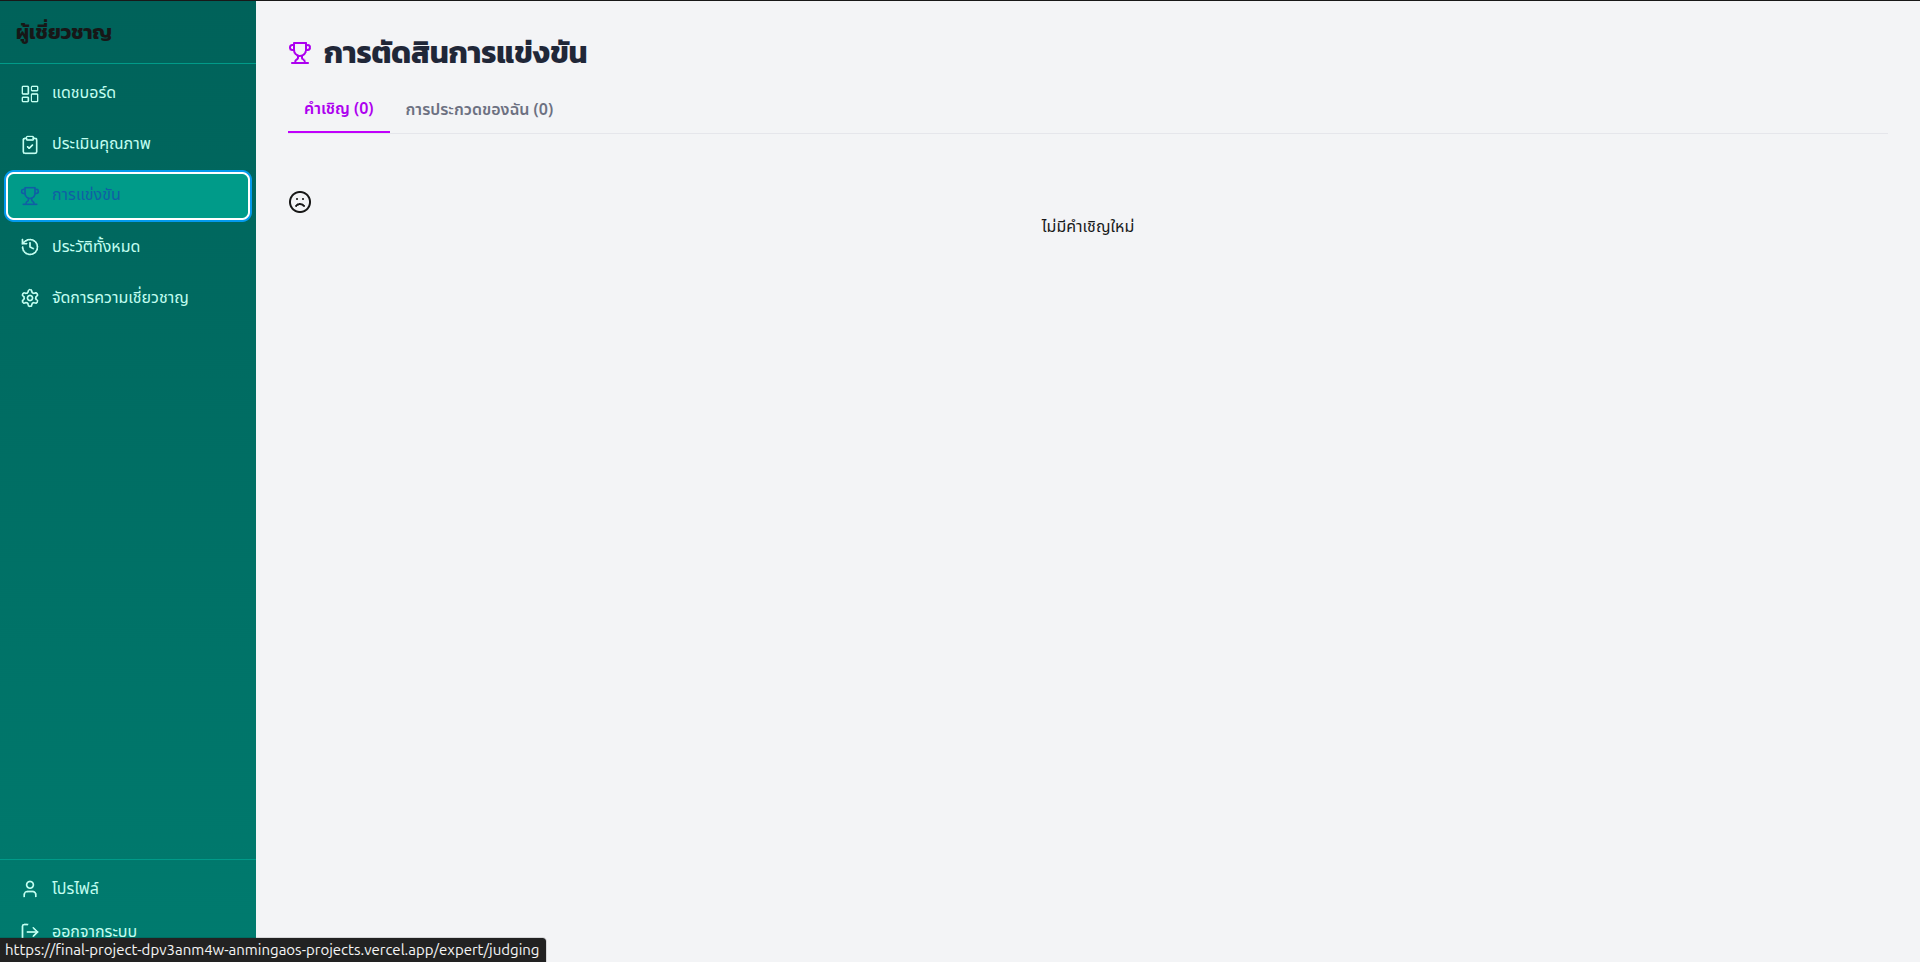
\includegraphics[width=0.8\linewidth]{EP3}
	\caption{หน้าห้องตัดสิน — รายการปลาที่ต้องให้คะแนน}
\end{figure}

\noindent{\bfseries\fontsize{16pt}{19.2pt}\selectfont วิธีใช้งานหน้าห้องตัดสิน — รายการปลาที่ต้องให้คะแนน}\par

\begin{sloppypar}
	\begin{enumerate}
		\item หน้าแสดงรายชื่อปลาที่ต้องให้คะแนนของการแข่งขันแต่ละรายการ หากผู้จัดการยังไม่เปิดสถานะ “ตัดสิน” ระบบจะแจ้งว่า “ยังไม่เปิดการตัดสิน”
		\item แสดงการ์ดปลา: รูปแรก ชื่อปลา ชื่อผู้ส่ง ปุ่ม “ให้คะแนน” และเช็กบ็อกซ์ “เปรียบเทียบ”
		\item แถบควบคุมด้านบนบอกจำนวน “เลือกไว้: X/10” พร้อมปุ่ม “เปรียบเทียบ” และ “ล้างการเลือก”
		\item โหมดเปรียบเทียบ: แสดงปลาที่เลือกแบบกริด เลือกเลื่อนรูปได้ (ปุ่มลูกศร/ภาพย่อ) และกรอก “คะแนนรวม (0–100)” แบบ Quick Score ต่อแต่ละตัว
		\item ปุ่ม “บันทึกคะแนนที่กรอก” จะบันทึกเฉพาะคะแนนรวม (โหมด Quick) ของรายการที่กรอกตัวเลขไว้
		\item ปุ่ม “ให้คะแนน” บนการ์ด จะเปิดฟอร์มให้คะแนนละเอียด (ScoringFormModal) เพื่อกรอกคะแนนตามเกณฑ์และส่งผล
		\item หลังบันทึกคะแนนหรือส่งคะแนนสำเร็จ ระบบจะแจ้งเตือน รีเฟรชรายการ และล้างการเลือกโดยอัตโนมัติ
		\item ปุ่ม “กลับไปหน้ารายการ” ใช้กลับไปหน้าเชิญตัดสิน/รายการแข่งขันของผู้เชี่ยวชาญ
	\end{enumerate}
\end{sloppypar}

\noindent{\bfseries\fontsize{16pt}{19.2pt}\selectfont ขั้นตอนใช้งาน}\par

\begin{sloppypar}
	\begin{enumerate}
		\item เข้าเมนูผู้เชี่ยวชาญ ไปยัง “ห้องตัดสิน — รายการปลาที่ต้องให้คะแนน”
		\item หากขึ้นข้อความ “ยังไม่เปิดการตัดสิน” ให้รอผู้จัดการเปลี่ยนสถานะ แล้วกดรีเฟรชเพื่อโหลดใหม่
		\item ให้คะแนนแบบละเอียด (แนะนำ)
		\begin{enumerate}
			\item เลือกปลาที่ต้องการ แล้วกด “ให้คะแนน”
			\item กรอกคะแนนตามหัวข้อในฟอร์ม และกด “ส่งคะแนน”
		\end{enumerate}
		\item ให้คะแนนแบบรวดเร็ว (Quick Score) หลายตัวพร้อมกัน
		\begin{enumerate}
			\item ติ๊ก “เปรียบเทียบ” ที่การ์ดปลา (เลือกได้สูงสุด 10 ตัว) แล้วกด “เปรียบเทียบ”
			\item ในหน้าต่างเปรียบเทียบ เลื่อนดูรูป (ลูกศร/ภาพย่อ) และกรอก “คะแนนรวม (0–100)” ต่อแต่ละตัว
			\item กด “บันทึกคะแนนที่กรอก” เพื่อบันทึกเฉพาะคะแนนรวมของรายการที่มีตัวเลข
		\end{enumerate}
		\item ต้องการล้างการเลือก กด “ล้างการเลือก” ที่แถบควบคุมหรือในหน้าต่างเปรียบเทียบ
		\item เสร็จงานแล้ว กด “กลับไปหน้ารายการ” เพื่อย้อนกลับไปยังหน้ารวมการตัดสิน
	\end{enumerate}
\end{sloppypar}


\begin{figure}[h]
	\centering
	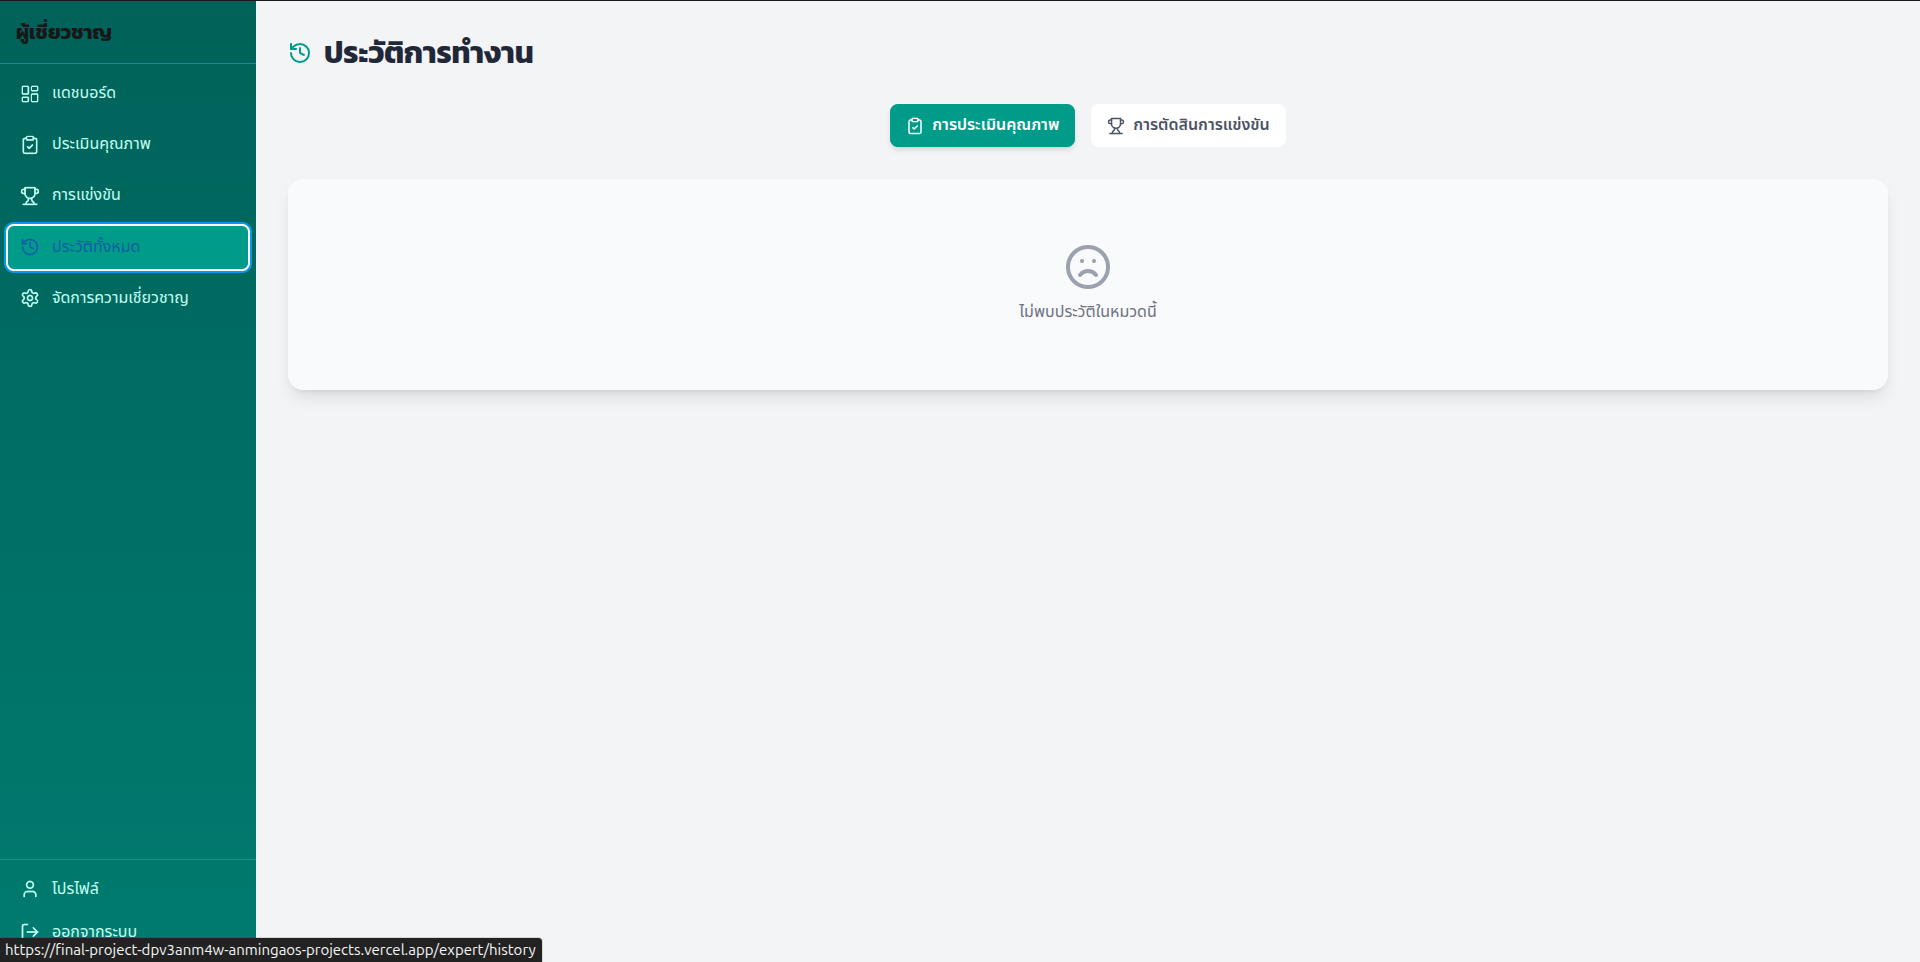
\includegraphics[width=0.8\linewidth]{EP4}
	\caption{หน้า “ประวัติการทำงานผู้เชี่ยวชาญ”}
\end{figure}

\noindent{\bfseries\fontsize{16pt}{19.2pt}\selectfont วิธีใช้งานหน้า “ประวัติการทำงานผู้เชี่ยวชาญ”}\par
\begin{sloppypar}
	\begin{enumerate}
		\item หน้าสรุปผลงานที่เคยทำ แบ่ง 2 หมวด: \textit{การตัดสินการแข่งขัน} และ \textit{การประเมินคุณภาพ} (สลับด้วยปุ่มแท็บด้านบน)
		\item ระบบแสดงตารางตามหมวดที่เลือก: ชื่อปลา/ชื่อการแข่งขัน, เจ้าของ/ชื่อปลา, ประเภท, คะแนนรวม, วันที่เสร็จสิ้น
		\item คะแนนจะแสดงทศนิยม 2 ตำแหน่ง; หากเป็นหมวดประเมินคุณภาพและรายการยังไม่ “ประเมินแล้ว” จะแสดง “–”
		\item วันที่แสดงในรูปแบบไทยอัตโนมัติ; หากข้อมูลไม่สมบูรณ์จะแสดง “–”
		\item มีสถานะโหลดและหน้าว่าง (Empty State) เมื่อไม่มีข้อมูลในหมวดนั้น ๆ
		\item ระบบจำหมวดล่าสุดที่เลือกไว้ (บันทึกในเบราว์เซอร์) กลับมาเปิดอีกครั้งจะอยู่ที่หมวดเดิม
	\end{enumerate}
\end{sloppypar}

\noindent{\bfseries\fontsize{16pt}{19.2pt}\selectfont ขั้นตอนใช้งาน}\par
\begin{sloppypar}
	\begin{enumerate}
		\item เปิดเมนู “ประวัติการทำงาน” ของผู้เชี่ยวชาญ
		\item เลือกหมวดที่ต้องการดู:
		\begin{enumerate}
			\item “การตัดสินการแข่งขัน” — ดูประวัติให้คะแนนในเวทีประกวด
			\item “การประเมินคุณภาพ” — ดูประวัติการตรวจคุณภาพรายปลา
		\end{enumerate}
		\item ตรวจรายการในตาราง:
		\begin{enumerate}
			\item ตรวจชื่อปลา/ชื่อการแข่งขัน และเจ้าของ/ชื่อปลา (ตามหมวด)
			\item ดูประเภทและคะแนนรวม (ทศนิยม 2 ตำแหน่ง)
			\item ตรวจวันที่เสร็จสิ้นของงานนั้น ๆ
		\end{enumerate}
		\item หากไม่พบข้อมูล ระบบจะแสดงข้อความ “ไม่พบประวัติในหมวดนี้” ให้สลับหมวดหรือกลับมาภายหลัง
		\item ออกจากหน้าได้ทันที — ระบบจะจดจำหมวดที่เลือกไว้สำหรับการใช้งานครั้งถัดไป
	\end{enumerate}
\end{sloppypar}